
\subsection{Tiny Recursive Model (TRM)}

TRM è un'architettura di rete neurale introdotta da Jolicoeur-Martineau \cite{trm}, sviluppata a partire dalle idee alla base dell'Hierarchical Reasoning Model (HRM).

L'obiettivo principale è realizzare un modello capace di affrontare problemi che richiedono processi di ragionamento articolati, mantenendo al contempo un'architettura compatta e un numero contenuto di parametri.

TRM riprende alcuni dei principi introdotti da HRM, in particolare l'elaborazione ricorsiva e la supervisione iterativa, proponendone una versione semplificata.

Il cambiamento principale consiste nell'eliminazione della struttura gerarchica composta da due reti distinte, sostituite da un'unica rete neurale di piccole dimensioni, riutilizzata più volte durante il processo di elaborazione.

L'idea alla base del modello è che, anziché aumentare la profondità della rete introducendo ulteriori livelli e parametri, sia possibile riutilizzare gli stessi componenti attraverso più iterazioni. In questo modo, il modello può elaborare progressivamente le informazioni, mantenendo una rappresentazione interna del ragionamento e aggiornando la propria predizione.

\subsubsection{Contesto applicativo e risultati}

TRM è stato sviluppato e valutato su diverse tipologie di problemi, caratterizzate dalla necessità di individuare soluzioni attraverso l'elaborazione di configurazioni strutturate. Gli esperimenti presentati nel paper considerano principalmente tre ambiti: la risoluzione di Sudoku, la ricerca di percorsi all'interno di labirinti e i benchmark ARC-AGI.

In particolare, il modello viene valutato sul dataset Sudoku-Extreme, composto da griglie 9$\times$9 particolarmente difficili, e su Maze-Hard, che comprende labirinti 30$\times$30 nei quali è necessario individuare un percorso tra un punto di partenza e uno di arrivo.

Vengono inoltre considerati ARC-AGI-1 e ARC-AGI-2, benchmark costituiti da problemi di ragionamento visivo e astratto. In questi problemi, il sistema deve individuare le trasformazioni che collegano alcune coppie di griglie di esempio e applicarle a nuovi input, generando la configurazione di output corretta.

I risultati ottenuti mostrano come un modello relativamente piccolo possa raggiungere prestazioni competitive in problemi di questo tipo. In particolare, la variante TRM basata su MLP, composta da circa 5 milioni di parametri, raggiunge un'accuratezza dell'87,4\% su Sudoku-Extreme. La variante basata su self-attention, composta da circa 7 milioni di parametri, ottiene invece l'85,3\% su Maze-Hard, il 44,6\% su ARC-AGI-1 e il 7,8\% su ARC-AGI-2.

Questi risultati superano quelli ottenuti da HRM sugli stessi benchmark, pur utilizzando un numero significativamente inferiore di parametri. Il lavoro evidenzia quindi il potenziale delle architetture ricorsive compatte nell'affrontare problemi complessi, senza fare necessariamente affidamento su modelli di grandi dimensioni \cite{trm}.

\subsubsection{Implementazione tecnica}

L'implementazione originale di TRM è stata realizzata in Python, utilizzando PyTorch come framework principale per la definizione delle architetture neurali, la gestione dei tensori e l'esecuzione delle operazioni di addestramento e inferenza.

Il codice sfrutta inoltre CUDA per l'esecuzione delle operazioni computazionalmente intensive su GPU. Tra le librerie utilizzate figurano einops, per la manipolazione delle rappresentazioni tensoriali, e Hydra e OmegaConf, per la gestione della configurazione degli esperimenti. Per il monitoraggio delle fasi di addestramento viene inoltre utilizzato Weights \& Biases.

L'architettura implementata comprende componenti tipiche delle moderne reti neurali, tra cui RMSNorm per la normalizzazione, Rotary Positional Embeddings per la codifica posizionale e SwiGLU come funzione di attivazione. A seconda del problema affrontato, il modello può utilizzare meccanismi di self-attention oppure componenti MLP per l'elaborazione delle informazioni.

Il codice sorgente e le configurazioni utilizzate per gli esperimenti sono stati resi disponibili dagli autori in un repository pubblico, consentendo di analizzare e riprodurre l'implementazione descritta nel paper \cite{trmcode}.

\subsubsection{Differenze rispetto a HRM}

La principale differenza tra TRM e HRM riguarda la struttura utilizzata per realizzare il processo ricorsivo.

HRM utilizza due reti distinte, denominate High-Level Module e Low-Level Module, che operano a frequenze differenti e aggiornano due rappresentazioni latenti. TRM elimina questa separazione, utilizzando un'unica rete neurale condivisa per svolgere entrambe le operazioni.

Questa semplificazione comporta anche un cambiamento nell'interpretazione degli stati interni del modello. Le due rappresentazioni mantenute da TRM non vengono più interpretate come livelli gerarchici differenti, ma come elementi con funzioni complementari:

\begin{itemize}
    \item \textbf{Stato latente (\(z\)):} rappresenta le informazioni interne utilizzate dal modello durante il processo di ragionamento. Viene aggiornato ripetutamente e conserva informazioni elaborate nelle iterazioni precedenti.
    \item \textbf{Predizione corrente (\(y\)):} rappresenta la soluzione proposta dal modello in un determinato momento dell'elaborazione. Viene progressivamente aggiornata utilizzando le informazioni contenute nello stato latente.
\end{itemize}

Un'altra differenza riguarda il processo di addestramento. HRM utilizza un'approssimazione del gradiente a singolo passaggio, giustificata attraverso l'ipotesi di convergenza degli stati latenti verso un punto fisso. TRM supera questa impostazione, propagando il gradiente attraverso un intero processo ricorsivo. In questo modo non è necessario assumere che gli stati abbiano raggiunto un punto fisso per poter effettuare l'aggiornamento dei parametri.

Nel complesso, TRM mantiene il principio del ragionamento ricorsivo introdotto da HRM, ma ne semplifica la struttura, riducendo il numero di reti e introducendo un processo di aggiornamento più diretto.

\subsubsection{Architettura generale}

L'architettura di TRM è composta da pochi elementi fondamentali: una componente di embedding dell'input, una rete neurale ricorsiva, uno stato latente, una rappresentazione della predizione e alcune componenti di output.

Dato un input \(x\), questo viene inizialmente trasformato in una rappresentazione numerica attraverso un livello di embedding. Il modello utilizza inoltre due rappresentazioni iniziali: \(y\), che contiene una prima ipotesi della soluzione, e \(z\), che rappresenta lo stato latente iniziale.

La rete ricorsiva viene quindi applicata ripetutamente, riutilizzando gli stessi parametri. In particolare, il processo si articola in due operazioni:

\begin{enumerate}
    \item Aggiornamento dello stato latente \(z\), utilizzando l'input \(x\), la predizione corrente \(y\) e lo stato latente precedente.
    \item Aggiornamento della predizione \(y\), utilizzando la rappresentazione corrente della predizione e lo stato latente appena elaborato.
\end{enumerate}

Indicando con \(f_\theta\) la rete neurale ricorsiva, le due operazioni possono essere rappresentate attraverso le seguenti espressioni:

\[
    z^{(i+1)} = f_\theta(x, y, z^{(i)})
\]

\[
    y' = f_\theta(y, z^{(n)})
\]

dove \(n\) indica il numero di aggiornamenti dello stato latente effettuati prima di procedere alla revisione della predizione. La notazione evidenzia che la stessa rete viene utilizzata in entrambe le operazioni, ricevendo informazioni differenti in ingresso.

La sequenza descritta costituisce un ciclo ricorsivo completo: lo stato latente viene aggiornato più volte e, successivamente, viene utilizzato per migliorare la predizione corrente. Il processo può essere ripetuto ulteriormente, utilizzando i nuovi valori di \(y\) e \(z\) come punto di partenza per il ciclo successivo.

Al termine dell'elaborazione, la rappresentazione \(y\) viene convertita in una predizione attraverso una componente denominata output head, che trasforma la rappresentazione interna in valori utilizzabili per produrre il risultato finale.

Come illustrato in Figura~\ref{fig:trm_architecture}, la stessa rete viene riutilizzata nei diversi passaggi, consentendo di aggiornare progressivamente entrambe le rappresentazioni.

\subsubsection{Ricorsione e aggiornamento degli stati latenti}

La ricorsione rappresenta l'elemento centrale dell'architettura TRM. A differenza delle reti neurali tradizionali, nelle quali l'elaborazione avviene principalmente attraverso una successione di livelli distinti, TRM riutilizza ripetutamente la stessa rete per aggiornare le proprie rappresentazioni interne.

Durante un ciclo ricorsivo, il modello esegue inizialmente \(n\) aggiornamenti consecutivi dello stato latente \(z\). A ogni iterazione, la rete utilizza l'input originale, la predizione corrente e lo stato latente precedente per produrre una nuova rappresentazione.

Una volta completati questi aggiornamenti, lo stato latente viene utilizzato per modificare la predizione \(y\). Quest'ultima può quindi essere interpretata come la soluzione attualmente proposta dal modello, mentre \(z\) conserva le informazioni elaborate durante il processo di ragionamento.

Il ciclo completo può essere ripetuto per un numero \(T\) di volte. In questo modo, il modello può approfondire progressivamente l'elaborazione, senza introdurre nuovi parametri a ogni iterazione.

Un aspetto importante è che la ricorsione non consiste nella semplice ripetizione di una predizione: a ogni passaggio vengono aggiornate entrambe le rappresentazioni, permettendo al modello di utilizzare le informazioni precedentemente elaborate per migliorare il risultato.

\subsubsection{Deep supervision}

Un ulteriore elemento fondamentale di TRM è rappresentato dalla deep supervision, un meccanismo che permette di supervisionare il modello attraverso più passaggi successivi.

Durante il processo di addestramento, anziché elaborare ciascun esempio attraverso un unico ciclo ricorsivo, il modello ripete il processo di aggiornamento per un numero massimo di \(N_{\text{sup}}\) passaggi di supervisione.

Al termine di ciascun passaggio, la predizione prodotta viene confrontata con il risultato atteso attraverso una funzione di perdita. I parametri della rete vengono quindi aggiornati utilizzando il gradiente calcolato durante l'elaborazione.

Gli stati \(y\) e \(z\) vengono mantenuti e utilizzati come inizializzazione del passaggio successivo. In questo modo, il modello non riparte da una rappresentazione iniziale a ogni iterazione, ma continua a elaborare le informazioni già acquisite, affinando progressivamente la propria predizione.

Il meccanismo permette quindi di aumentare la profondità effettiva dell'elaborazione senza dover costruire una rete composta da un numero elevato di livelli distinti.

Il paper introduce inoltre una distinzione tra i cicli ricorsivi eseguiti all'interno di un singolo passaggio di supervisione. In particolare, i primi \(T-1\) cicli vengono eseguiti senza calcolo dei gradienti, mentre l'ultimo viene eseguito mantenendo il grafo computazionale necessario alla backpropagation.

Questa scelta consente di migliorare gli stati interni attraverso più cicli ricorsivi, limitando al contempo il costo della propagazione del gradiente. A differenza di HRM, il gradiente viene comunque calcolato attraverso l'intero ultimo ciclo ricorsivo, senza ricorrere all'approssimazione a singolo passaggio basata sul punto fisso.

\subsubsection{Adaptive Computation Time e criteri di arresto}

Il modello introduce anche un meccanismo di calcolo adattivo, denominato Adaptive Computation Time (ACT), che permette di interrompere anticipatamente il processo di supervisione durante l'addestramento.

La motivazione deriva dal costo computazionale associato all'esecuzione di un numero fisso di passaggi per ogni esempio. Alcuni input possono infatti richiedere più iterazioni per ottenere una predizione corretta, mentre altri possono raggiungere una soluzione adeguata in un numero inferiore di passaggi.

Per gestire questa situazione, TRM utilizza una componente aggiuntiva, denominata Q-head, che riceve la rappresentazione corrente della predizione e stima la probabilità che il risultato sia già corretto.

Durante l'addestramento, questa componente viene supervisionata attraverso una funzione di perdita binaria (Binary Cross-Entropy), confrontando la propria predizione con l'effettiva correttezza del risultato prodotto dal modello.

Il valore restituito dalla Q-head viene quindi utilizzato per determinare se interrompere anticipatamente il processo di supervisione. Quando il valore supera la soglia prevista, il modello considera raggiunto un risultato sufficientemente affidabile e interrompe le ulteriori iterazioni. Rimane comunque definito un numero massimo di passaggi, che impedisce al processo di proseguire indefinitamente.

Rispetto alla soluzione adottata in HRM, TRM semplifica il meccanismo di arresto eliminando la necessità di un'ulteriore valutazione della rete per stimare il beneficio di una nuova iterazione. La decisione viene infatti appresa direttamente attraverso la previsione della Q-head, riducendo il costo computazionale associato all'ACT.

È importante sottolineare che, nell'implementazione originale, ACT viene utilizzato durante il training per ridurre il numero di passaggi di supervisione necessari per ciascun esempio. Durante la valutazione, invece, vengono eseguiti tutti i passaggi previsti, senza applicare l'interruzione anticipata.

\subsubsection{Considerazioni sull'architettura}

TRM propone quindi un approccio al ragionamento basato sulla ripetizione di una rete di piccole dimensioni, che aggiorna progressivamente una rappresentazione interna e una predizione corrente.

La combinazione tra ricorsione, deep supervision e calcolo adattivo permette di ottenere una maggiore profondità effettiva mantenendo contenuta la complessità dell'architettura. Il modello rappresenta pertanto un'alternativa alle reti più profonde e articolate, nelle quali l'aumento della capacità computazionale viene ottenuto principalmente attraverso l'introduzione di ulteriori parametri e livelli.

Queste caratteristiche costituiscono la base architetturale del progetto sviluppato in questa tesi, nel quale TRM viene adattato al gioco del Go attraverso una diversa rappresentazione dell'input e una componente di output specifica per la previsione delle mosse.

\begin{figure}[H]
    \centering
    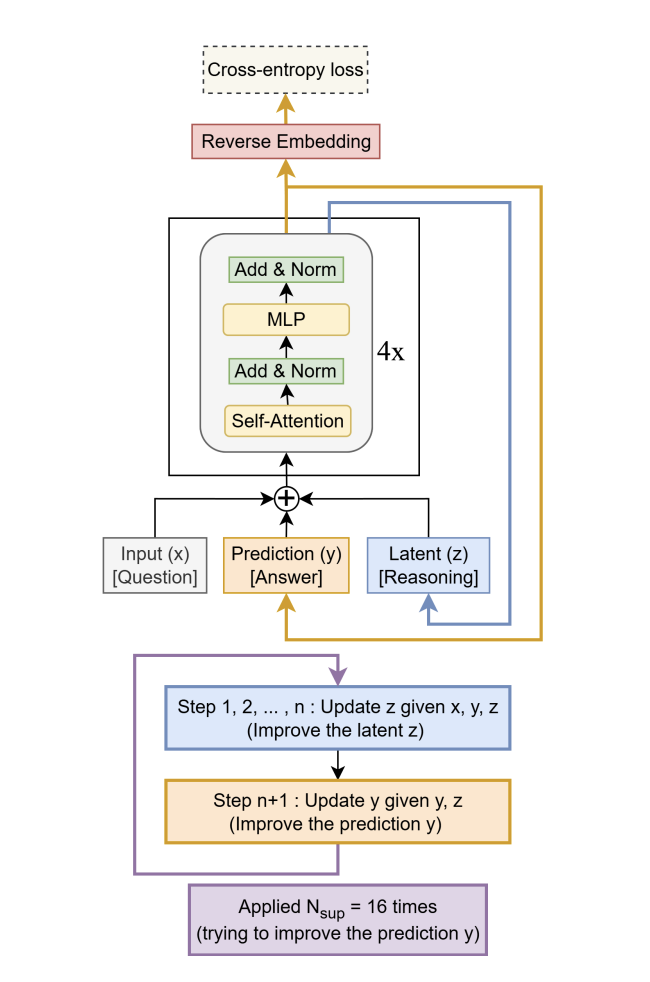
\includegraphics[width=0.75\textwidth]{img/trm_paper.png}
    \caption{Architettura del Tiny Recursive Model (TRM).
        Fonte: \cite{trm}.}
    \label{fig:trm_architecture}
\end{figure}
